
\chead{CHAPITRE 1. CADRE GÉNÉRAL DU PROJET}
\chapter{ Cadre général du projet }

%\renewcommand{\mtctitle}{Sommaire}
\setcounter{mtc}{2}
\minitoc

\newpage
\section*{Introduction}

\addcontentsline{toc}{section}{\protect\numberline{}Introduction}
\par L'analyse de la situation actuelle est grandement influencée par l'étude préliminaire, qui se concentrera sur la définition des besoins. Ce chapitre couvre le cadre général du projet, en présentant brièvement l'organisme d'accueil, notre application web de recrutement intégrant un système de parsing de CV basé sur spaCy NLP et un scoring automatique, ainsi que la méthode de conduite de projet et les outils logiciels employés.

\vspace*{-0.5cm}

\section{Cadre du projet}
\hspace{0.5cm} \textbf Ce projet s'inscrit dans le cadre du travail de fin d'études en vue de l'obtention du diplôme de licence professionnelle en Business Computing, spécialité Business Information System, à ESPRIT School of Business (ESB), au cours de l'année universitaire 2024/2025. Ce stage a été effectué au sein de l'entreprise PwC TAC Tunisie, sous la supervision de Mme. Yoldez El Gaaloul, où nous avons développé une application web de recrutement intégrant des technologies intelligentes de parsing de CV et de scoring automatique.
\vspace*{-0.5cm}

\section{Présentation de l'organisme d'accueil}
Fondée en 1998 et implantée à Tunis, \textbf{PwC TAC Tunisie} est une filiale du réseau mondial PricewaterhouseCoopers, leader dans les services d'audit, de conseil et de fiscalité. Elle propose des solutions sur mesure dans les domaines de l'audit financier, du conseil en management et des services technologiques, au profit des entreprises locales et internationales opérant en Tunisie. Se distinguant par son engagement envers l'innovation et la transformation digitale, PwC TAC Tunisie constitue également un environnement privilégié pour le développement des jeunes talents au sein d'un réseau professionnel de renommée mondiale.

\vspace{0.3cm}
\begin{figure}[H]
\centering

\includegraphics[width=7cm, height=5cm]{Figures/PwC_logo.png}
\caption{Logo de la société "PriceWaterhouseCoopers TAC Tunisie"}\cite{beecoders_logo}
\end{figure}

\vspace{0.1cm}

\section{Etude de l'existant}
L'automatisation des processus de recrutement est devenue une nécessité incontournable pour les entreprises souhaitant optimiser leur gestion des ressources humaines. L'objectif de cette étude est d'analyser les solutions actuellement disponibles sur le marché afin d'identifier leurs forces et leurs limites, et ainsi justifier la nécessité d'un outil innovant tel que SmartRec. Ce dernier se distingue par son approche intelligente, intégrant des technologies de traitement du langage naturel (NLP via SpaCy) pour le parsing automatique des CVs des candidats, ainsi qu'un système de scoring automatisé permettant d'évaluer objectivement chaque candidat sur une échelle de 100 points, offrant ainsi aux recruteurs une expérience de gestion des candidatures plus efficace et plus précise.



\subsection{Description de l'existant}
Les solutions RH disponibles sur le marché, telles que \textbf{LinkedIn Jobs}, \textbf{Workday} et \textbf{Taleo}, demeurent insuffisantes dans une perspective globale. LinkedIn Jobs se limite à la publication d'offres, Workday reste coûteux et complexe, tandis que Taleo souffre d'une interface obsolète et d'un manque de fonctionnalités intelligentes. Aucune de ces plateformes n'exploite réellement l'intelligence artificielle pour optimiser les processus RH, ce qui justifie pleinement la création de \textbf{SmartRec}.

\subsection{Critique de l'existant }
Avant d'entamer le développement de SmartRec, il est primordial d'explorer le paysage concurrentiel existant, afin de mieux cerner les avantages et les insuffisances des outils déjà disponibles sur le marché. Cette analyse permet de s'appuyer sur les bonnes pratiques existantes tout en proposant des fonctionnalités distinctives et une réelle valeur ajoutée pour les recruteurs et les candidats.
\subsubsection{Linkedin}
 
LinkedIn Jobs est une plateforme mondiale de recrutement en ligne, spécialisée dans la mise en relation entre recruteurs et candidats. Elle permet aux entreprises de publier des offres d'emploi, de consulter les profils des candidats et de gérer les candidatures reçues grâce à une interface web intuitive et des outils de recherche avancés.
 \cite{esperoo2025}
\vspace{0.3cm}

\begin{figure}[H]
\centering
\fbox{
\includegraphics[width=3cm, height=3cm]{Figures/logo_linkedin.png}}
\caption{Logo de site web "Linkedin"}\cite{logo_linkedin}
\label{SEIF}
\end{figure}



\vspace{0.1cm}
Voici ce que nous avons pu observer comme points forts et points à améliorer dans cette application.
\vspace{0.2cm}
\\
\\
\par \underline{\textbf{Points Forts}}\\

\begin{itemize}[label=\textbullet]

 \item[\ding{51}] \textbf{Suivi précis du temps de travail :}LinkedIn Jobs se distingue par sa capacité à connecter les recruteurs avec des millions de candidats à travers le monde, offrant ainsi un accès à une base de données étendue de profils professionnels variés et qualifiés.
 
\item[\ding{51}] \textbf{Planification optimisée :} Elle facilite la publication d'offres d'emploi claires et ciblées, adaptées aux besoins et aux exigences de chaque entreprise.

\item[\ding{51}]  \textbf{Interface locale :} La plateforme est adaptée aux besoins des entreprises de toutes tailles, qu'elles soient locales ou internationales, grâce à ses outils de recrutement flexibles et personnalisables.

\end{itemize}

\par \underline{\textbf{Points Faibles}}\\
\begin{itemize}[label=\textbullet]

\item[\ding{56}]  \textbf{Absence de fonctionnalités intelligentes : } Aucun système de parsing automatique des CVs ni de scoring automatisé des candidats n'est intégré, ce qui oblige les recruteurs à évaluer manuellement chaque candidature reçue.

\item[\ding{56}]  \textbf{Absence de gestion des candidatures avancée :} Il n'est pas possible de filtrer, classer ou scorer automatiquement les candidats selon leurs compétences et leur adéquation avec le poste proposé.
\item[\ding{56}]  \textbf{Absence de gestion des CVs :} Il n'existe pas d'espace dédié au stockage et à l'analyse automatique des CVs des candidats, ce qui complique la consultation et le suivi des dossiers de candidature par les recruteurs.

\end{itemize}

\subsubsection{Workday Recruiting}
Workday Recruiting est une solution SaaS mondiale de gestion du recrutement, intégrée au sein de la suite RH de Workday. Elle propose un système automatisé pour la publication des offres d'emploi et la gestion des candidatures, avec un suivi des candidats et un tableau de bord centralisé permettant aux recruteurs de piloter efficacement leur processus de recrutement.

\cite{WorkDay}
\vspace{0.3cm}

\begin{figure}[H]
\centering
\fbox{
\includegraphics[width=11cm, height=2cm]{Figures/workday_logo.png}}
\caption{Logo de platform "WorkDay" }\cite{workday_logo}
\label{fig:planification}
\end{figure}



\vspace{0.2cm}
Voici ce que nous avons pu observer comme points forts et points à améliorer dans cette application.

\par \underline{\textbf{Points Forts}}\\
\begin{itemize}[label=\textbullet]
\item[\ding{51}]  \textbf{Facilité d'utilisation :} La plateforme dispose d'une interface claire et ergonomique, ce qui permet aux recruteurs et aux responsables RH de la prendre en main rapidement et sans difficultés.
\item[\ding{51}]  \textbf{Automatisation du processus de recrutement : } Le suivi des candidatures est fluide et structuré, avec des notifications automatiques envoyées aux recruteurs et aux candidats, assurant ainsi une traçabilité complète de chaque étape du processus de recrutement.
\item[\ding{51}]  \textbf{Adapté aux grandes entreprises :} Sa mise en œuvre rapide et ses fonctionnalités avancées en font une solution bien adaptée aux entreprises de grande taille souhaitant optimiser et centraliser leur processus de recrutement.
\end{itemize}

\par \underline{\textbf{Points Faibles}}\\
\begin{itemize}[label=\textbullet]
\item[\ding{56}]  \textbf{Absence de fonctionnalités intelligentes : }Aucune fonctionnalité liée au parsing automatique des CVs ou au scoring automatisé des candidats n'est disponible, ce qui oblige les recruteurs à évaluer manuellement chaque dossier de candidature.
\item[\ding{56}]  \textbf{Absence d'analyse des candidats :}  La plateforme ne permet pas d'évaluer automatiquement les compétences, l'expérience ou le niveau d'adéquation des candidats par rapport au poste proposé.
\item[\ding{56}]  \textbf{Manque de flexibilité : } L'outil reste limité dans ses options de personnalisation et ne s'adapte pas facilement aux besoins spécifiques de chaque entreprise en matière de recrutement.

\end{itemize}

\subsubsection{ Taleo  }
Taleo est une plateforme de recrutement américaine développée par Oracle, reconnue mondialement et utilisée par de nombreuses entreprises de grande taille. Elle permet de centraliser la gestion des offres d'emploi, le suivi des candidatures et la gestion des talents, grâce à une interface complète et des outils performants dédiés aux équipes RH.
\cite{Taleo}
\vspace{0.3cm}

\begin{figure}[H]
\centering
\fbox{
\includegraphics[width=3cm, height=3cm]{Figures/Taleo_logol.jpg}}
\caption{Logo de platform "NGES RH"}\cite{Taleo_logo}
\label{fig:planification}
\end{figure}

\vspace{0.2cm}
Voici ce que nous avons pu observer comme points forts et points à améliorer dans cette application.

\par \underline{\textbf{Points Forts}}\\
\begin{itemize}[label=\textbullet]
\item[\ding{51}]  \textbf{Gestion complète du recrutement :} La plateforme assure une prise en charge intégrale des différentes étapes du processus d'embauche, allant de la diffusion des offres d'emploi jusqu'à la sélection finale des candidats les plus qualifiés.
\item[\ding{51}]  \textbf{Déploiement à l'échelle mondiale: } Il est conforme aux exigences réglementaires tunisiennes (ex. : CNSS, bulletins de paie).La plateforme est utilisée par des entreprises dans de nombreux pays, ce qui lui permet de s'adapter aux différentes exigences et aux contextes variés des organisations à travers le monde.
\item[\ding{51}]  \textbf{Disponibilité d'un module de recrutement avancé :} La plateforme intègre un système complet de gestion des candidatures, offrant aux recruteurs un suivi détaillé et structuré de chaque candidat tout au long du processus de sélection.
\end{itemize}

\par \underline{\textbf{Points Faibles}}\\
\begin{itemize}[label=\textbullet]
\item[\ding{56}]  \textbf{Fonctionnalités de recrutement limitées : } Bien que la plateforme dispose d'un module de recrutement, celui-ci reste insuffisant car il ne propose ni parsing automatique des CVs, ni scoring automatisé des candidats, ni analyse intelligente des dossiers de candidature.
\item[\ding{56}]  \textbf{Manque de collaboration entre recruteurs : } La plateforme ne permet pas aux membres de l'équipe RH de partager des avis, d'échanger des commentaires ou de travailler conjointement sur l'évaluation des candidats.
\item[\ding{56}]  \textbf{Interface utilisateur complexe:} Taleo possède une interface vieillissante et peu intuitive, nécessitant une formation approfondie, ce qui ralentit le processus de recrutement.
\end{itemize}

\subsection{Solution proposée:}
C’est précisément pour pallier l’ensemble de ces insuffisances que SmartRec a été
conçu. Ce projet ambitionne de fournir une solution moderne, intelligente et adaptée aux
exigences du marché actuel. À la différence des outils existants, fréquemment cantonnés à
une fonctionnalité unique ou dépourvus d’innovation technologique, SmartRec rassemble
en une seule plateforme cohérente et performante l’ensemble des services indispensables à
une gestion efficace du recrutement. Plusieurs éléments fondamentaux distinguent SmartRec de la concurrence :

\textbullet \hspace{0.2cm} \textbf {recrutement intelligent et optimisé : } SmartRec propose un module exhaustif couvrant la publication des offres, la réception des candidatures ainsi qu'un mécanisme de sélection automatisé reposant sur un scoring avancé et une analyse approfondie des CVs.

\textbullet \hspace{0.2cm} \textbf{ collaboration active au sein des équipes RH : } la plateforme offre un environnement de travail collaboratif permettant aux recruteurs de partager leurs évaluations, d'échanger leurs retours et de statuer collectivement sur les profils des candidats.



\textbullet \hspace{0.2cm} \textbf{Une exploitation réelle de l'intelligence artificielle:} contrairement aux solutions concurrentes, SmartRec intègre l'IA au cœur de ses processus afin d'automatiser l'analyse des dossiers, d'affiner le scoring des candidats et d'améliorer la qualité des décisions de recrutement.

\textbullet \hspace{0.2cm} \textbf{Sécurité et ergonomie : } un contrôle rigoureux des accès selon les rôles des utilisateurs, associé à une interface fluide, réactive et intuitive, garantit une expérience utilisateur optimale.



\subsection{Justification du choix d’un site web de Recrutement}

Dans un contexte professionnel marqué par des mutations profondes et continues, la transformation numérique des fonctions RH s'est progressivement imposée comme un impératif stratégique pour toute organisation aspirant à renforcer son efficacité opérationnelle et à consolider sa position concurrentielle. Le déploiement d'une plateforme web spécialisée dans la gestion des ressources humaines constitue dès lors une démarche innovante et résolument tournée vers l'avenir, offrant la possibilité de regrouper l'ensemble des opérations RH au sein d'un dispositif unique et intégré. Une telle centralisation présente des avantages multiples et significatifs : elle permet notamment d'automatiser des tâches administratives répétitives et chronophages, à l'instar de la gestion des absences, du suivi des présences ou de la conduite du processus de recrutement, contribuant ainsi à réduire considérablement les risques d'erreurs humaines tout en permettant aux équipes de se consacrer pleinement à des activités à plus forte valeur ajoutée. En outre, ce type de solution favorise une communication interne plus fluide et transparente, en donnant aux collaborateurs comme aux responsables RH un accès simplifié et structuré aux informations dont ils ont besoin. Elle représente également un gage de conformité aux obligations légales et réglementaires en vigueur. C'est animé par ces convictions que SmartRec a été développé, avec la volonté affirmée de proposer une solution complète, ergonomique et performante, capable d'accompagner durablement les entreprises dans la valorisation et la gestion optimale de leur capital humain.



\section{Méthodologie adoptée}
\par 
La réussite d'un projet informatique ne saurait se réduire aux seuls choix technologiques opérés, mais repose fondamentalement sur la qualité de son pilotage et la rigueur de son organisation. Une conduite de projet véritablement efficace implique une vision stratégique clairement définie, une démarche structurée et réfléchie, ainsi que des décisions fondées sur des données concrètes et fiables. C'est dans cette perspective que le développement de SmartRec a été mené en adoptant la méthodologie Scrum, reconnue pour sa clarté et sa simplicité de mise en œuvre. De façon générale, il est possible de distinguer deux grandes familles de méthodologies de conduite de projet :
	\begin{itemize}[label=\textbullet]
\textbullet \hspace{0.2cm} \textbf {Les approches traditionnelles ou prédictives : } ces méthodes reposent sur une planification exhaustive et séquentielle établie en amont, où chaque étape est définie avant le lancement du projet, offrant ainsi peu de marge pour d'éventuels ajustements en cours de développement\\
\textbullet \hspace{0.2cm} \textbf {Les méthodes agiles : } à l'inverse, ces approches privilégient la flexibilité, l'interaction permanente entre les membres de l'équipe et l'amélioration continue du produit, permettant une adaptation rapide et efficace face aux évolutions et aux besoins émergents.
    \end{itemize}



\subsection{Méthodes classiques}
Les méthodes classiques telles que le modèle en cascade et le cycle en V reposent sur une logique séquentielle stricte, où chaque phase doit être achevée avant de passer à la suivante. Bien qu'elles offrent un cadre structuré, leur rigidité et leur manque de flexibilité les rendent inadaptées aux projets nécessitant des ajustements fréquents et une évolution continue.
\subsubsection{Présentation des méthodes classiques }
Les méthodes classiques, également désignées sous le terme de méthodes prédictives, se caractérisent par une planification minutieuse établie en amont et une exécution strictement linéaire du projet. Ce dernier progresse de manière séquentielle à travers des phases bien définies, à savoir l'analyse, la conception, le développement, les tests et le déploiement, chacune devant être intégralement finalisée avant d'entamer la suivante. Parmi les approches les plus répandues, on distingue :

\textbullet \hspace{0.2cm} \textbf{Le cycle en V :} largement utilisé en informatique, il repose sur une validation systématique à chaque étape, garantissant une traçabilité rigoureuse mais imposant une structure particulièrement inflexible.

\textbullet \hspace{0.2cm} \textbf{La méthode Waterfall :} fondée sur une progression unidirectionnelle, cette approche ne permet aucun retour en arrière une fois une phase achevée, la rendant adaptée uniquement aux projets aux exigences stables et bien définies.

\textbullet \hspace{0.2cm} \textbf{Les méthodes PERT et Gantt :} outils de planification complémentaires, le diagramme de Gantt visualise l'enchaînement des tâches dans le temps, tandis que PERT permet d'identifier les chemins critiques et d'anticiper les risques de retard.
    
\subsubsection{Insuffisances des approches traditionnelles }
 
En dépit de leur cadre organisationnel structuré, les méthodes classiques révèlent plusieurs insuffisances majeures lorsqu'elles sont confrontées aux exigences des projets modernes et évolutifs. Parmi les faiblesses les plus significatives, on peut relever :
	
	\begin{itemize}[label=\textbullet]
	\item	\textbf{Une rigidité contraignante :  }difficile d’adapter le projet en cours de route si les besoins changent.
    \item \textbf{Une visibilité tardive du produit :} Le produit final n’est visible qu’à la fin, ce qui peut générer des écarts par rapport aux attentes.
    
    \item \textbf{Une détection différée des anomalies :} Les erreurs découvertes en fin de cycle sont coûteuses à corriger.
    \item	\textbf{Des échanges limités au sein de l'équipe :}les échanges entre les équipes sont limités, ce qui freine l’adaptation et l’innovation.

    \item	\textbf{Une déconnexion des attentes réelles:} les spécifications sont parfois déconnectées des attentes des utilisateurs finaux.



	\end{itemize}

 \subsection{Naissance des approches agiles }
Afin de saisir pleinement l'engouement croissant des organisations pour les méthodes agiles, il convient de remonter aux fondements historiques qui ont présidé à leur émergence. C'est en février 2001 que dix-sept experts reconnus du développement logiciel se sont réunis à Snowbird, dans l'Utah aux États-Unis, animés par la volonté commune de repenser les pratiques existantes et de dépasser les limites inhérentes aux méthodes traditionnelles. De cette rencontre fondatrice est né le célèbre Manifeste Agile, qui a posé les valeurs cardinales de l'agilité :

	\begin{itemize}[label=\textbullet]
	\item La primauté des interactions humaines sur les processus formalisés et les outils techniques,
 	\item Un logiciel opérationnel plutôt qu'une documentation exhaustive et figée,
    \item Une relation de confiance avec le client qui prime sur les contraintes contractuelles,
 	\item La capacité d'adaptation aux changements qui l'emporte sur le respect rigide d'un plan préétabli.
		\end{itemize}
        \vspace{0.2cm}
		\par Ce manifeste fondateur s'appuie également sur douze principes directeurs promouvant la transparence, l'autonomie des équipes, la livraison rapide et continue de valeur, ainsi que la satisfaction permanente du client. Depuis lors, les méthodes agiles ont connu une diffusion remarquable, s'étendant bien au-delà de la sphère informatique pour irriguer l'ensemble des domaines de la gestion de projet.



\subsection{Choix de méthodologie : SCRUM} 
Dans le domaine du développement logiciel, plusieurs méthodes agiles ont émergé pour rendre la gestion de projet plus souple et mieux adaptée aux besoins réels des utilisateurs. Bien qu’elles reposent sur les mêmes valeurs, chaque méthode a ses spécificités et ses avantages. Parmi les plus répandues, on retrouve :

\textbullet \hspace{0.2cm} \textbf{ Scrum : }articulée autour de cycles itératifs courts appelés sprints, cette méthode instaure une organisation rigoureuse des rôles et favorise une livraison régulière de valeur.

\textbullet \hspace{0.2cm} \textbf{XP (Extreme Programming) :} orientée vers l'excellence technique, elle privilégie des pratiques telles que les tests automatisés et l'intégration continue afin de garantir la qualité du code produit.

\textbullet \hspace{0.2cm} \textbf{Kanban :} reposant sur une représentation visuelle des flux de travail, elle assure un suivi continu et transparent de l'avancement des tâches via un tableau dynamique.

\begin{table}[H]
\begin{center}
\captionsetup{justification=centering}
 \caption{\label{tab:<< Tableau comparatif – Méthodes agiles >>} Tableau comparatif des méthodes agiles  }
\begin{tabular}{|p{2cm}|p{7.5cm}|p{6.5cm}|} \arrayrulecolor{black}\rowcolor{WhiteSmoke}
\hline 
\textbf{Méthode} &
\hspace*{1.5cm} \textbf{Points Forts} &
 \hspace*{1cm} \textbf{Points Faibles} \\ \hline
\textbf{SCRUM} &
  \begin{tabular}[c]{@{}l@{}}• Organisation claire des rôles (Product \\ Owner, Scrum Master, équipe).\\ •Progression visible grâce aux sprints \\itératifs \\ • Communication fluide et ajustements \\réguliers \end{tabular} &
  \begin{tabular}[c]{@{}l@{}}• Peut devenir contraignant si les \\rôles ne sont pas rigoureusement\\ respectés.\\• Nécessite une équipe \\préalablement formée à la méthode. \end{tabular} \\ \hline
\textbf{XP} &
  \begin{tabular}[c]{@{}l@{}}• Privilégie une qualité élevée du code.\\• Intégration systématique de tests\\ automatisés \\• Encourage la collaboration étroite entre \\développeurs.
  \end{tabular} &
  \begin{tabular}[c]{@{}l@{}}• Exige un niveau technique avancé\\ et une grande rigueur.\\•  Peu adapté aux équipes \\nombreuses ou aux environnements\\ très formalisés.\end{tabular} \\ \hline
\textbf{Kanban} &
  \begin{tabular}[c]{@{}l@{}}• Mise en place simple et rapide. \\• Visualisation intuitive via un tableau de \\bord. \\• Grande souplesse et réactivité face aux\\ imprévus. \end{tabular} &
  \begin{tabular}[c]{@{}l@{}}• N'impose aucune structure\\ temporelle ni itérative.\\•Offre une vision globale\\ insuffisante pour les projets\\ complexes.\end{tabular} \\ \hline
\end{tabular}

\end{center}
\end{table}
L'examen du tableau comparatif révèle que Scrum constitue le choix le plus judicieux pour \textbf{SmartRec}. Kanban, bien que souple, manque de cadre structurant, tandis que XP privilégie la technique au détriment des besoins fonctionnels. Scrum offre ainsi un équilibre optimal entre rigueur organisationnelle, clarté des rôles et capacité d'adaptation, répondant parfaitement aux exigences de notre projet.


\subsection{SCRUM}
Jouissant d'une popularité considérable au sein de l'écosystème du développement logiciel, Scrum se distingue parmi les approches agiles par la clarté de son cadre méthodologique et la robustesse de ses résultats. Pour en saisir pleinement la portée et les enjeux, il apparaît indispensable d'en examiner les éléments constitutifs, en parcourant ses principes fondateurs jusqu'aux mécanismes concrets qui régissent son application au quotidien au sein d'une équipe projet.

\subsubsection{Présentation de Scrum} 

\par Scrum est un cadre de travail agile reposant sur une organisation itérative et incrémentale, découpant le travail en cycles courts appelés sprints, dont la durée varie généralement entre une et quatre semaines. Fondé sur trois piliers fondamentaux que sont la transparence, l'inspection et l'adaptation, il favorise une livraison continue de fonctionnalités opérationnelles tout en permettant à l'équipe de s'ajuster rapidement aux évolutions des besoins. Cette approche instaure ainsi un environnement de travail collaboratif, structuré et propice à l'amélioration continue du produit développé.\\

 


\vspace*{-0.5cm}
\subsubsection{Concepts de SCRUM}
\hspace{1.5cm}\textbf Scrum s'articule autour de trois composantes essentielles intimement liées. Premièrement, les rôles, comprenant le Product Owner qui définit les priorités et gère le backlog, le Scrum Master qui facilite le processus et lève les obstacles, et l'équipe de développement qui réalise les fonctionnalités. Deuxièmement, les artefacts, constitués du Product Backlog regroupant l'ensemble des fonctionnalités à développer, du Sprint Backlog listant les tâches sélectionnées pour chaque sprint, et de l'incrément représentant la version fonctionnelle livrée à l'issue de chaque cycle. Troisièmement, les cérémonies, encompassing le Sprint Planning pour la planification, le Daily Scrum pour la synchronisation quotidienne, la Sprint Review pour la démonstration du travail accompli et la Sprint Retrospective pour l'amélioration continue du processus.


\subsubsection{Acteurs dans SCRUM} 
Scrum s'articule autour de trois composantes fondamentales et complémentaires, qui structurent l'ensemble du cadre méthodologique et garantissent son bon fonctionnement:
 \begin{itemize}[label=\textbullet]
 \item 	\textbf{Le Product Owner}   définit les priorités et gère le backlog produit
  \item \textbf{Le Scrum Master} facilite le processus et lève les obstacles
  \item \textbf{L’équipe de développement,} réalise les tâches et livre les fonctionnalités
\end{itemize}

\subsubsection{Terminologie Scrum}
\begin{itemize}[label=\textbullet]
  \item \textbf{ Product backlog : } liste priorisée de toutes les fonctionnalités du produit
  \item \textbf{ User Stories : } description concise d'une fonctionnalité exprimée du point de vue de l'utilisateur final afin de refléter ses besoins réels.
  \item \textbf{  Sprint :}  cycle de développement itératif et timeboxé au terme duquel une version fonctionnelle du produit est livrée.
 \item \textbf{Sprint Planning :} planification des tâches du sprint
 \item \textbf{Daily Scrum :} réunion quotidienne de synchronisation
 \item \textbf{Sprint Backlog :} liste des tâches sélectionnées pour un sprint.
 \item \textbf{Sprint Review :} démonstration du travail accompli.
 \item \textbf{Sprint Retrospective :} analyse et amélioration du processus.


 \end{itemize}
 
\subsubsection{Processus SCRUM} 
\hspace{0.5cm}\textbf La méthodologie Scrum repose sur une démarche itérative et incrémentale, au sein de laquelle le projet progresse à travers une succession de sprints organisés et structurés. Chaque sprint débute par une phase de planification au cours de laquelle l'équipe sélectionne les éléments prioritaires du Product Backlog à réaliser, puis s'achève par une revue et une rétrospective permettant d'évaluer le travail accompli et d'améliorer continuellement le processus. 



La figure ci-après illustre le déroulement global du processus Scrum. 


\begin{figure}[H]
\centering
\fbox{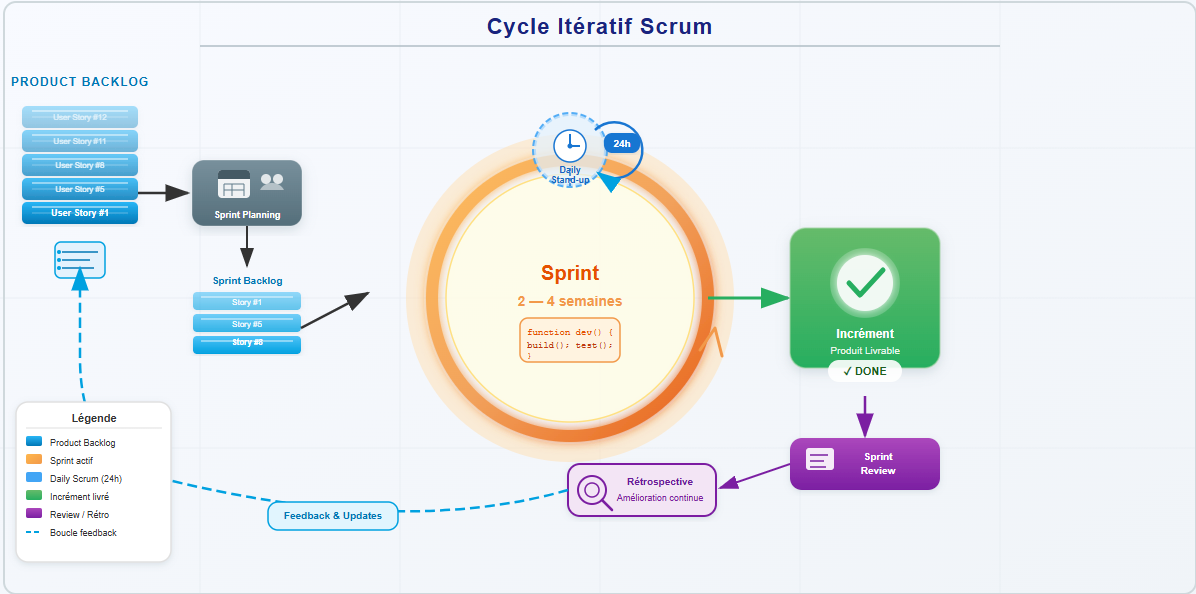
\includegraphics[width=15cm, height=7cm]{Figures/deroulement scrum.png}}
\caption{Déroulement de scrum}\cite{scrum_process_figure}
\label{fig:planification}
\end{figure}

Dans le cadre du développement de SmartRec, la méthodologie Scrum a été mise en œuvre à travers une succession de sprints d'une durée fixe généralement comprise entre deux et quatre semaines, définie dès la phase de cadrage du projet. Cette dernière a permis de clarifier la vision globale de la plateforme, d'établir le backlog initial sous forme de tickets de tâches et de définir le planning général du développement. 

\par Chaque sprint s'est articulé autour de quatre étapes fondamentales :
\begin{itemize}[label=\textbullet]
\item \textbf{La planification du sprint}: en début de chaque sprint, l'équipe se réunissait afin de sélectionner les tickets prioritaires du backlog à traiter et d'identifier les tâches nécessaires à l'atteinte des objectifs fixés, le tout géré et suivi via l'outil \textbf{Trello}.

\item \textbf{Les mêlées quotidiennes (Daily Stand-ups)}: des réunions journalières courtes étaient tenues afin que chaque membre partage l'état d'avancement de ses travaux, ses prévisions et les éventuels obstacles rencontrés, favorisant ainsi une communication fluide et des ajustements rapides.


\item \textbf{La revue du sprint}: à l'issue de chaque sprint, un bilan des livrables produits était dressé afin de vérifier leur conformité aux objectifs initialement définis et d'affiner le backlog pour le sprint suivant.

\item \textbf{La rétrospective du sprint}: cette réunion interne visait à analyser le déroulement du sprint écoulé, à identifier les points positifs à consolider et les axes d'amélioration à exploiter pour optimiser les sprints suivants.


\end{itemize}

\section*{Conclusion} \addcontentsline{toc}{section}{\protect\numberline{}Conclusion}%
\hspace{0.5cm}\textbf
En guise de synthèse, ce chapitre introductif a permis d'établir les fondements conceptuels et méthodologiques du projet \textbf{SmartRec}, en présentant le contexte général et en analysant de manière critique les solutions RH existantes sur le marché. L'identification des lacunes et insuffisances des systèmes actuels a mis en lumière la nécessité de développer une plateforme web innovante, capable d'optimiser et de centraliser la gestion des ressources humaines. Par ailleurs, le recours à la méthodologie agile Scrum a été justifié par sa capacité à allier flexibilité, rigueur organisationnelle et adaptabilité tout au long du cycle de développement. Ce chapitre pose ainsi les jalons indispensables à la bonne conduite et à la réussite du projet dans les phases ultérieures.



%\addcontentsline{toc}{section}{\protect\numberline{}Conclusion}%
